\section{Work Completed}\label{section:work}

%This should discuss what progress has been made on designing, implementing and evaluating the artifact. Care must be taken to ensure that any discussion of technical points are clearly explained, with diagrams being used where appropriate.
%In many cases, the evaluation proper will not yet have begun. However, it is important to demonstrate that sufficient thought has been given to the evaluation.

% Consideration of test generation techniques used
% Trade off => Performance vs accuracy?
% Needed to create test cases that adhered to the pre-conditon

An implementation of the tool has been created with generation of core and more complex data types. 
The tool has also been extended to use integer range analysis to constrain input values generated for better performance. 
Unit tests have also been written to check the tool generates the values expected.

The tool can be executed via the command line with several arguments. To use the tool, a user must pass in the path of a WyIL file and specify the test case generation technique to use, number of tests they wish to generate and ranges for generating integer values. Ranges are used to limit the integers generated between an inclusive, minimum number and an exclusive, upper number.

% TODO example of the tool
%An example use of the tool would be to execute:
%\texttt{}

Whiley's interpreter is used to validate inputs and outputs from tests. Valid inputs are based on verifying pre-conditions and constraints on the input type used. Only valid inputs are used in tests. A successful test is checked by verifying outputs with the function's post-conditions and constraints on the outputs' type.

% These invalid inputs should be discarded and replaced by generating new input data.

Currently, only functions within the program with a post-condition can be tested as they can be verified.

\subsection{Test Case Generation Techniques}

QuickCheck for Whiley currently employs random test-case and exhaustive test case generation to generate test cases: 

\subsubsection{Random Test Case Generation}

A fixed number of tests determined by the user is randomly generated. Previous inputs are not considered which may lead to the same inputs being generated.
Knuth's Algorithm S from \cite{artProgv2} was considered to generate unique inputs to solve this problem but has not been implemented yet.

\subsubsection{Exhaustive Test Case Generation}
A fixed number of tests determined by the user are exhaustively generated, where ranges are used to limit integers and the size of arrays during generation. This is so that a feasible number of combinations can be generated. Integers are generated starting from the lower limit. Arrays are generated starting from the smallest possible array size, which is usually an empty array.

\subsection{Data types generated}
Different generators are created for the different types defined in Whiley. 
Figure \ref{fig:qc-generators} illustrates the structure of the generators used.
Each generator generates a value. It also has a size for the number of input combinations and \texttt{resetCount()} and \texttt{exceedCount()} methods for monitoring input combinations generated for test-case generation.
 
\begin{figure}
	\caption{Class diagram of Generators in QuickCheck for Whiley}
	\label{fig:qc-generators}
	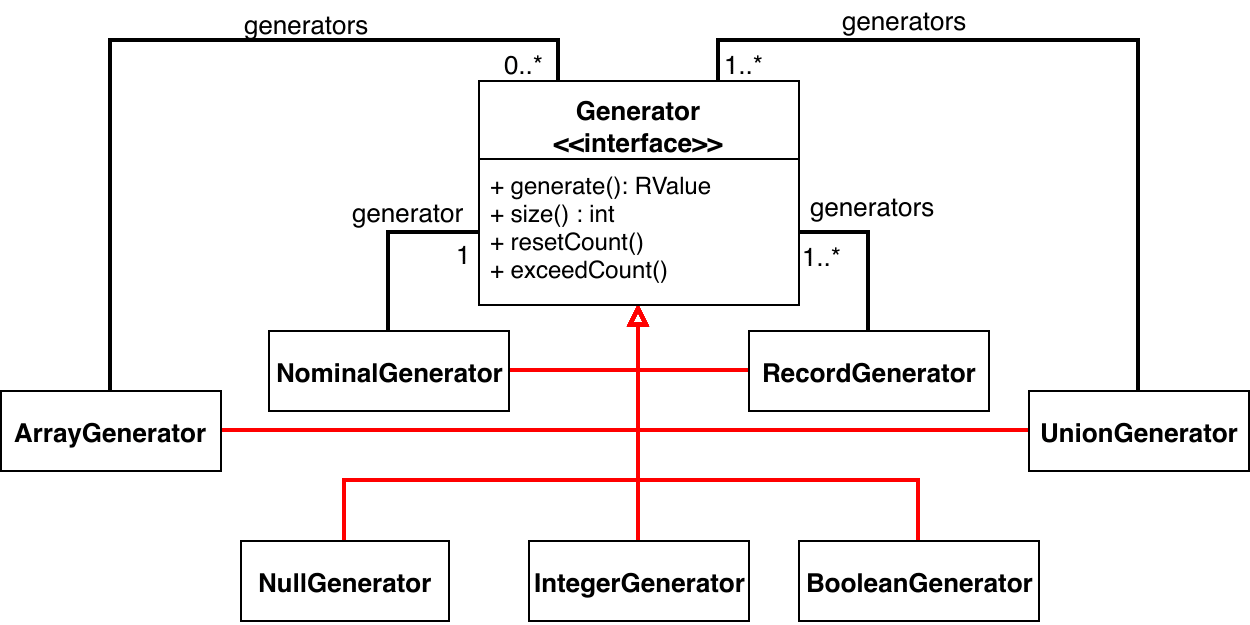
\includegraphics[width=\textwidth]{qc-generators}
	\centering
\end{figure}

\begin{description}
	\item[Null] Generate a \texttt{null} value.
	\item[Boolean] Generates a Boolean which is either \texttt{true} or \texttt{false}.
	\item[Integer] Generates an integer between a bounded range. This range may be modified based on constraints applied to the integer.
	\item[Array] Generates an array with a specific element type between a bounded size range.
	The size of arrays is currently limited to a maximum size of three elements due to the performance cost of generating larger arrays.
	\item[Nominal] A nominal represents a user-defined type by redefining a type with a different name \cite{WhileyLang}. Therefore, a generator for a nominal wraps a generator for a different type to generate a value. A nominal can also have a type constraint/invariant applied to it \cite{WhileyLang}.
	\item[Record] "A record type describes the set of all compound values made from one or more fields, each of which has a unique name and a corresponding type \cite{WhileyLang}." A closed record contains a fixed number of fields whereas an open record can have any number of fields with different types.
	A closed record is generated by generating values that correspond to each field. Generators corresponding to each field is required as each field may have different types. 
	Generation for open records has not been implemented as there can be an arbitrary number of fields added to a record. This could be a future extension to the tool.
	\item[Union] A union is made up of multiple types where the value can correspond to any one of the types declared. For example, the type \texttt{bool|int} can hold either a boolean or an integer value. 
	A union is generated by generating a value from one of the declared types. A generator corresponding to each type is required. 
	% Talk about fairness in union generation

	Values for the union type could be skewed towards generating values for only type. It was important that the different types for each union are generated fairly. Therefore, the union generator was implemented so that a value from a different type would be generated each time by iterating through the generators within the union generator.

\end{description}

\subsection{Integer Range Analysis}

Generating and checking for invalid inputs is costly in terms of performance. 
Therefore, it would be beneficial to reduce the number of invalid inputs generated to improve the performance of the tool.
One method to remove invalid inputs for integers is to shrink the ranges used during generation thus no longer generate invalid inputs.

For example, define the nominal type, \texttt{type nat is (int x) where x \textgreater= 0} and execute the tool for an integer range between -5 and 5. Invalid inputs are numbers below 0. An integer generator for this input will only generate numbers between 0 and 5, removing the need to generate then discard invalid inputs below 0.

This is implemented by evaluating the constraints within a nominal type to discover integer range generated from the constraint.
Existing code from \cite{whileyIntegerRangeCode} was used to create the integer ranges which is based off \cite{whileyIntegerRange}.
The discovered integer range is passed down in the nominal generator until it reaches the relevant integer or array generator where it is intersected with an existing range.
If the ranges are invalid, i.e. the lower range is greater than the upper range then an error is thrown.

Integer ranges are only applied to constraints that follow the format: \texttt{x op c} where \texttt{x} is the named variable in the nominal type, \texttt{op} is an operator out of the set \{\textgreater, \textless, \textgreater=, \textless=, \&\&, $||$, ==\} and \texttt{c} is a constant number.

\subsection{Evaluating the tool}
The tool has been evaluated by executing a variety of tests notably, the test suite for the Whiley Compiler containing tests for valid inputs and outputs and tests for invalid inputs and outputs \cite{whileyCompilerTests}. 
Valid tests should always pass for valid inputs whereas invalid tests should always fail for some valid input. 
A successful implementation of the tool should pass all tests.

To evaluate the Whiley Compiler test suite, the tool is executed twice using exhaustive test generation for each test. The first execution is with integer ranges between -5 (inclusive) and 0  (exclusive) whereas the second execution is for integer ranges between 0 (inclusive) and 5 (exclusive).
Currently, the tool passes 80.69\% (4 s.f) (422 out of 523 tests) of the valid tests and 93.49 (4 s.f.)\% (316 out of 338 tests) of the invalid tests \cite{qcWhileyStatistics}. Some of the tests may be falsely pass by the tool due to the small domain of integer ranges used. Therefore, some tweaking will be required to determine a suitable integer range across all tests.

% Talk about how the tool is run
% Talk about evaluating the tool using the Whiley valid and invalid tests
% How to evaluate the tool